\documentclass{article}

% -- Packages covering every feature area demonstrated individually --
\usepackage{amsmath}
\usepackage{amssymb}
\usepackage{enumitem}
\usepackage{booktabs}
\usepackage{multirow}
\usepackage{graphicx}
\usepackage{caption}
\usepackage{listings}
\usepackage{xcolor}
\usepackage{url}
\usepackage{hyperref}
\hypersetup{colorlinks=true, linkcolor=blue, urlcolor=magenta, citecolor=teal}

\lstset{
  basicstyle=\ttfamily\small,
  showstringspaces=false,
  frame=single,
  breaklines=true,
}

\title{The platex Kitchen Sink}
\author{platex demo}
\date{}

\begin{document}
\maketitle
\tableofcontents

\section{Introduction}
This single document exercises every feature demonstrated individually
elsewhere in this gallery: math, lists, tables, figures, bibliography,
sectioning, code listings, hyperlinks, and footnotes\footnote{Like this
one.} — all compiled through the same \texttt{compile()} call.

\section{Mathematics}
Euler's identity is famously compact:
\[
  e^{i\pi} + 1 = 0.
\]
It generalizes as part of a broader identity:
\begin{align}
  \sum_{n=1}^{\infty} \frac{1}{n^2} &= \frac{\pi^2}{6} \\
  \int_0^1 x^2 \, dx &= \frac{1}{3}
\end{align}
for all $x \in \mathbb{R}$.

\section{Lists}
\begin{itemize}
  \item Unordered items
  \begin{itemize}
    \item can nest
  \end{itemize}
  \item and stay tidy
\end{itemize}
\begin{enumerate}[label=(\alph*)]
  \item Ordered items
  \item with custom labels
\end{enumerate}

\section{Tables}
\begin{table}[h]
  \centering
  \begin{tabular}{l l r}
    \toprule
    Engine & Type & Speed \\
    \midrule
    pdflatex & Native TeX Live & Fast \\
    tectonic & Bundled fallback & Medium \\
    \bottomrule
  \end{tabular}
  \caption{Compilation engines supported by platex.}
  \label{tab:engines}
\end{table}
Table~\ref{tab:engines} lists the supported engines.

\section{Figures}
\begin{figure}[h]
  \centering
  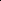
\includegraphics[width=3cm]{demo-figure.png}
  \caption{An image supplied via \texttt{CompileOptions.files}.}
  \label{fig:demo}
\end{figure}
See Figure~\ref{fig:demo} for the supplied asset.

\section{Code}
\begin{lstlisting}
import { compile } from 'platex';
const result = await compile(source, { bibliography: 'bibtex' });
\end{lstlisting}

\section{Citations}
LaTeX's model traces back to \TeX{} itself \cite{knuth1984texbook}, with
\cite{lamport1994latex} building the tooling most authors use, and cloud
editors like \cite{overleaf2023} making it collaborative. See
\url{https://overleaf.com} for one such editor.

\section{Conclusion}
Every rendering path above — math, structured text, tabular data, images,
external references, source code, and cross-references — passes through
the identical \texttt{compile()} entrypoint, whether resolved locally or
via a remote platex service.

\bibliographystyle{plain}
\bibliography{references}

\end{document}
